\documentclass[14pt]{extreport}
\usepackage{gost}
\usepackage{hyperref}
\usepackage{makecell}
\usepackage{ragged2e}
\usepackage{graphicx}%Вставка картинок правильная
\usepackage{float}%"Плавающие" картинки
\usepackage{wrapfig}%Обтекание фигур (таблиц, картинок и прочего)
	
\usepackage{lscape}
\justifying
\makeatletter
\@addtoreset{figure}{part}% Reset figure numbering at every part
\makeatother
\renewcommand{\thefigure}{\arabic{figure}}% Figure number is part.figure
\renewcommand{\thetable}{\arabic{table}}



%Тут можно вставить дополнительные пакеты

\begin{document}
\pagestyle{empty} %  выключаем нумерацию
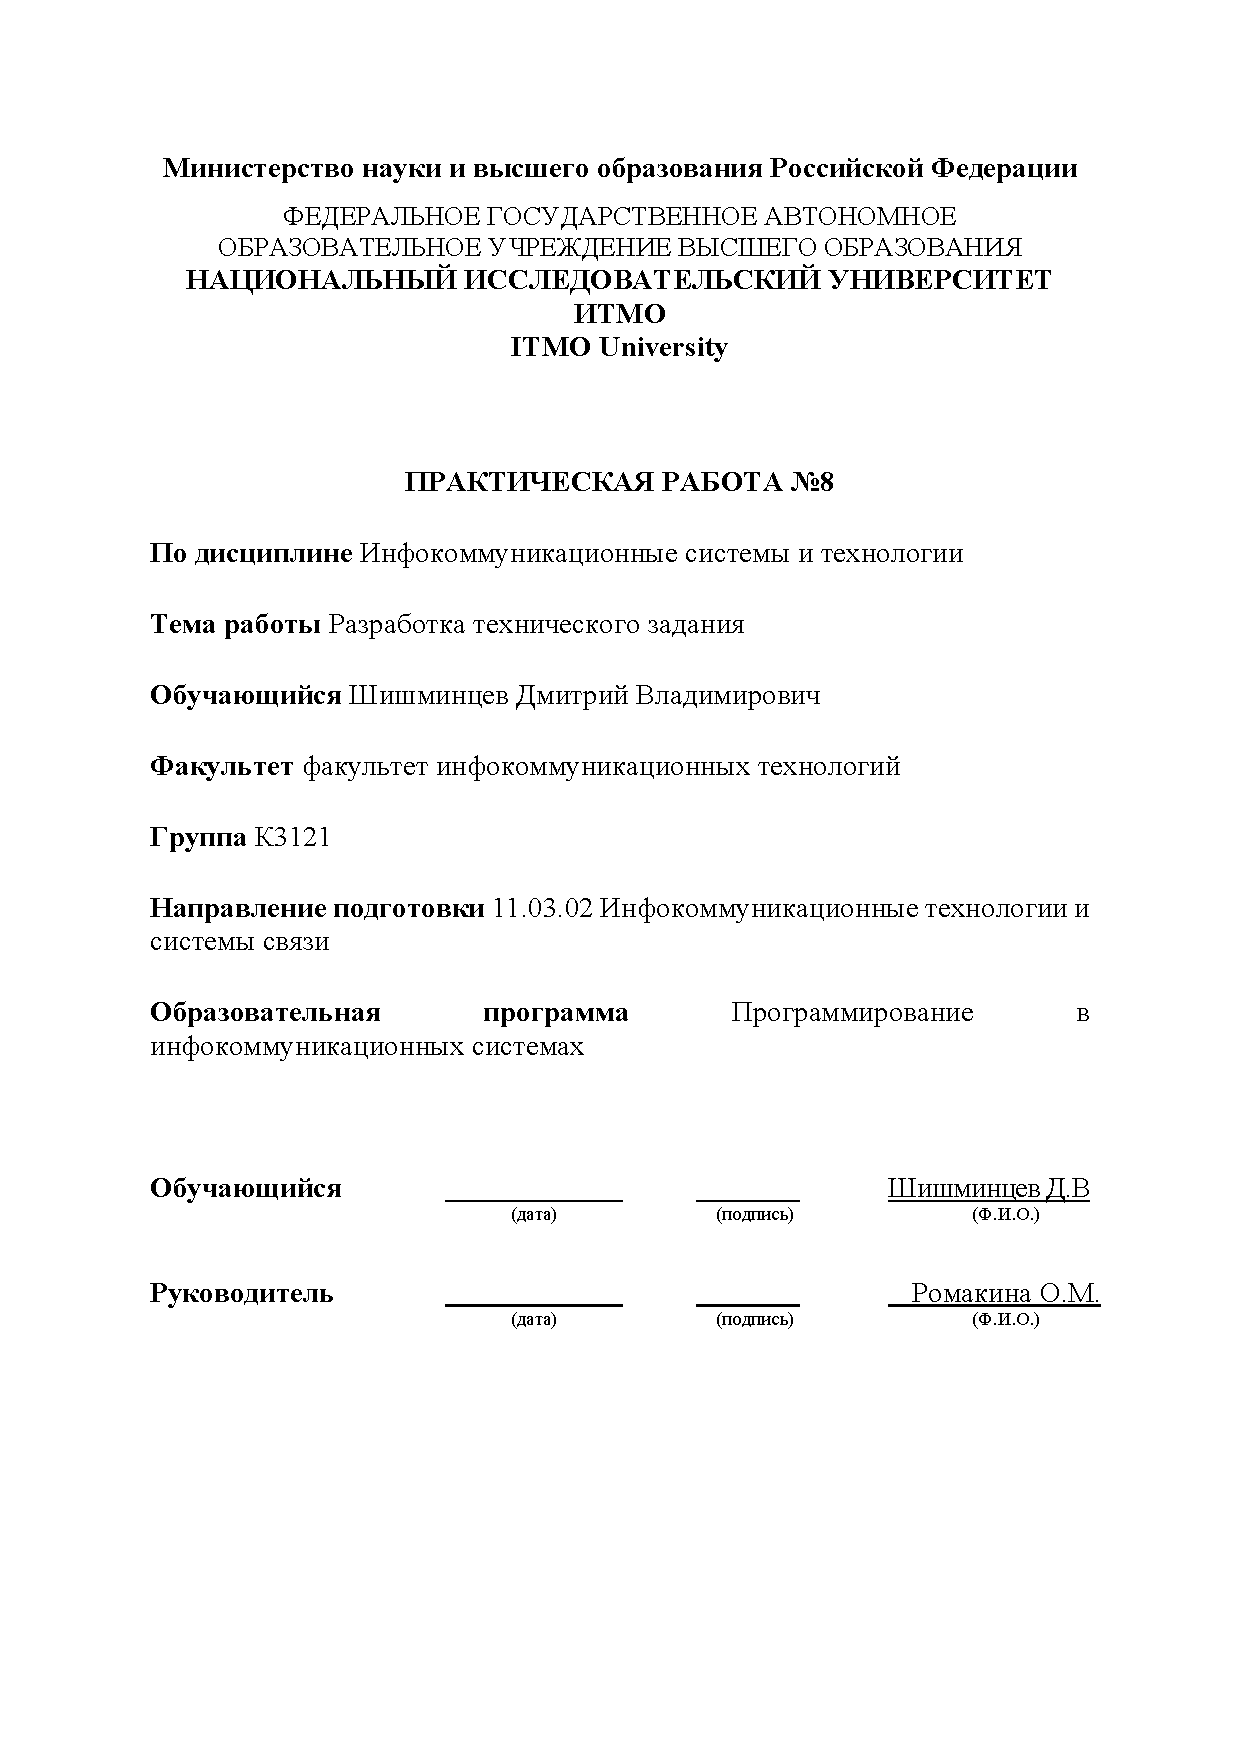
\includepdf[pages=-,pagecommand={}]{title_page.pdf}


\pagestyle{plain} % включаем нумерацию
\tableofcontents
\intro\label{intro} 

    Данная практическая работа содержит в разработанное техническое задание на создание инфокоммуникационной системы.


\chapter{Общие сведения}
    \section{Наименование инфокоммуникационной системы}
        Наименование разрабатываемого программного обеспечения: meet\textunderscore me. Выбранный регистр написания и специальные символы являются обязательными требованиями к использованию названия. 
    \section{Сроки начала и окончания работ по созданию инфокоммуникационной системы}
        После заключения договора с Заказчиком, исполнитель обязуется выполнить все работы по созданию инфокоммуникационной системы в течении 90 рабочих дней.

\chapter{Назначение и цели создания системы}
    \section{Назначение системы}
        Информационная система meet\textunderscore me предназначено для планирования встреч с друзьями и родственниками в виде календаря. 
        Система показывает пересечение свободного времени пользователя с одним или несколькими его друзьями.
        C помощью данной системы пользователь может эффективно планировать встречи со своими друзьями, родственниками или знакомыми.

    \section{Цели системы}
        Разрабатываемая  система имеет следующие цели:
        \begin{itemize}
            \item Учет пользовательского расписания
            \item Выявление пересечений расписания пользователя с другими пользователями 
            \item Планирование встреч с другими пользователями 
        \end{itemize}

\chapter{Характеристика объектов автоматизации}
        Объектом автоматизации является выявление пересечений расписания пользорвателя с другими пользователями посредством использование веб приложения.
        
        Веб приложение представляет из себя клиент-серверное приложение в виде веб-сайта для клиентской стороны, программного обеспечения работающего на сервеной части приложения, а так же системы управления базами данных.

\chapter{Требования к системе}

        \section{Требования к отказоустойчивости}
            Разрабатываемая инфокоммуникационная система должна быть отказоусточивой. Система должна выдерживать до 10000 одновременных пользователей. На всех уровнях обработки информации должна быть предусмотрена обработка ошибок. Действия обычного пользователя не должны выводить из строя систему. Необходимо предусмотреть возможные действия недобросовесных пользователей. 

        \section{Требования к интерфейсу}
            Разрабатываемый интерфейс должен быть построен согласно стилистическим нормам и должен быть максимально удобен для пользователя. Необходимо разработать интерфейсы следующих размеров (пикс.):
            \begin{itemize}
                \item 375x667
                \item 375x812 
                \item 390x844
                \item 414x896
                \item 810x1080
                \item 1280x720
                \item 1920x1080
                \item 2048x1080
                \item 3840x2160
            \end{itemize}

            Все интерфейсы должны выглядеть в едином стиле и иметь одинаковый функционал. Элементы управления системой должны быть расположены в интуитивно понятных для пользователя местах. Каждый элемент управления должен быть понятно обозначен и должен иметь лишь одну интерпретацию. Для системы следует разработать 2 цветовых гаммы, в светлых и темных тонах. Необходимо реализовать возможность быстро переключаться между цветовыми гаммами. Интерфейс должен выглядеть одинаково для следующих версий программного обеспечения:

            \begin{itemize}
                \item Google Chrome версии 57 или выше;
                \item Edge версии 16 или выше;
                \item Safari версии 11 или выше;
                \item Firefox версии 52 или выше; 
                \item Opera версии 44 или выше;
                \item Остальные браузеры на базе Chromium версии 57 или выше;
            \end{itemize}

            Поддержка семейства браузеров Internet Explorer не требуется. Для неподдерживаемого программного обеспечения необходимо уведомить пользователя о невозможности продолжения работы и предложить ему один из вариантов поддерживаемого программного обеспечения. 

            Интерфейс требуется реализовать в соответствии с представленным макетом интерфейса (Рисунок \ref{fig:d1}). 
            \begin{figure}[h]   
                \centering
                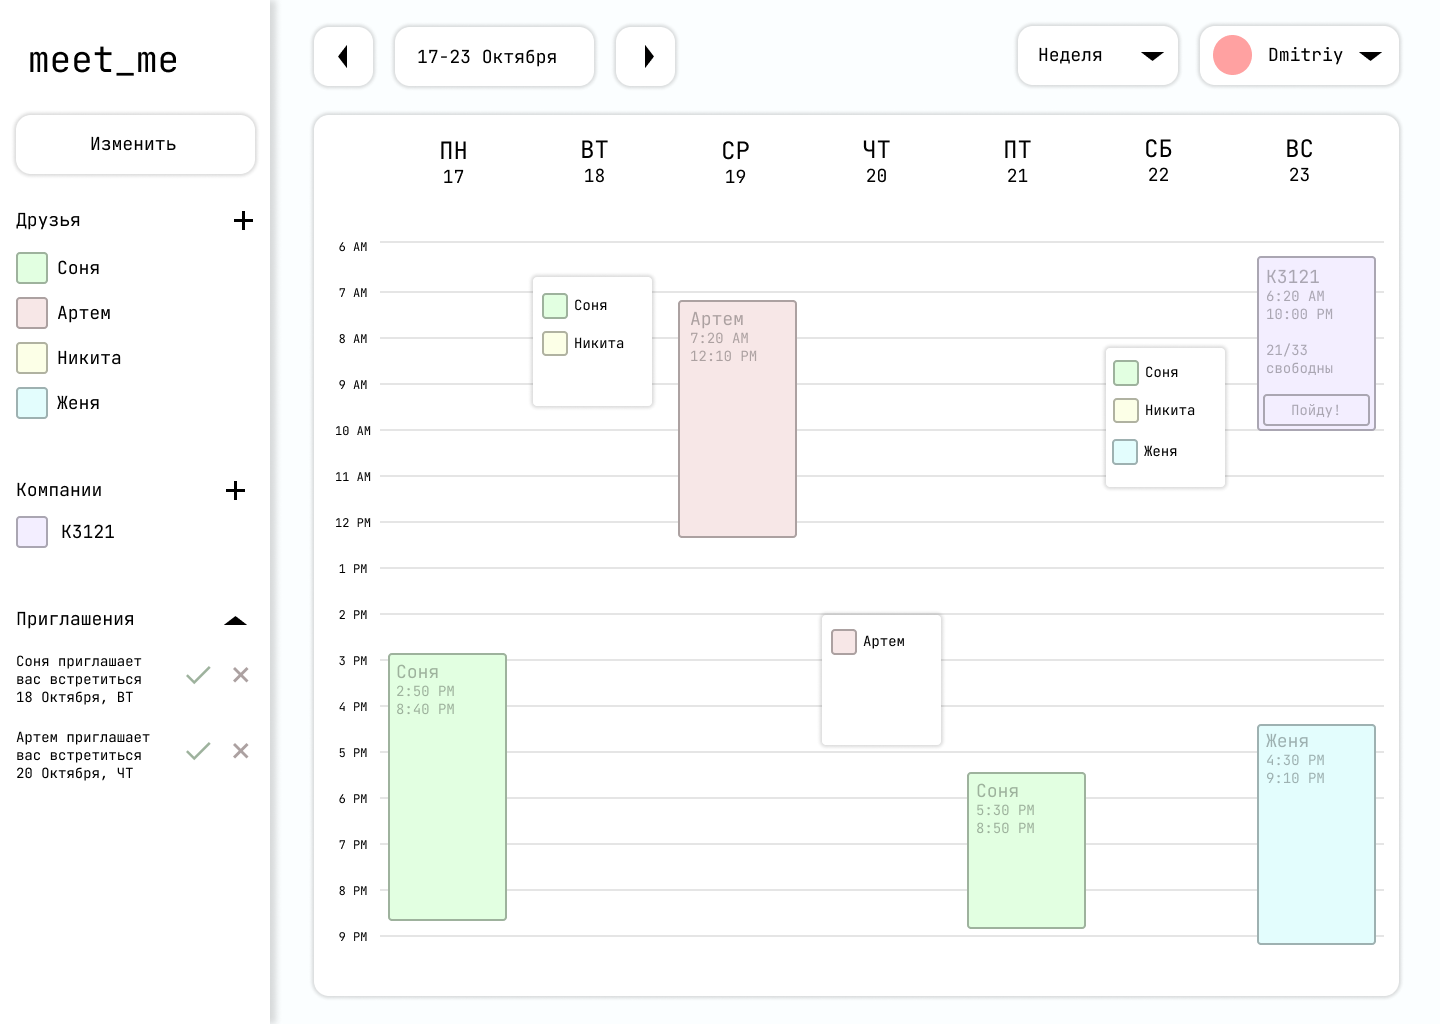
\includegraphics[width=0.9\linewidth]{./../lab3/prototype.png}
                \caption{ Прототип интерфейса}
                \label{fig:d1}
            \end{figure}
        \section{Требования к уровню безопасности}
            
            Для информационной системы требуется высокий уровень безопасности и защиты от несанкционированного доступа. Необходимо разработать механизмы двухфакторной аутентификации для пользователей с помощью генерации одноразовых паролей или аппаратных ключей. Необходимо отслеживать подозрительные попытки входа в аккаунт пользователя и своевременно уведомлять его об этом посредством e-mail. Предусмотреть действия недобросовесных пользователей такие как: SQL инъекции, внедрение вредоносного кода путем загрузки файлов, перебор паролей, многократные попытки входа и тд. 

        \section{Требования к программному обеспечению}

            В процессе разработки инфокоммуникационной системы необходимо использовать программное обеспечение с открытым исходным кодом и лицензиями MIT, BSD, GLP. В случае невозможности использовать программное обеспечение для той или иной задачи, необходимо согласовать с Заказчиком приобретение лицензии на проприетарное программное обеспечение и его дальнейшее использование. Для управлением базами данных требуется использование нереляционной системы управления базами данных. В качестве системы управления базами данных разрешается использовать проприетарное программное обеспечение MongoDB Enterpise версии 6.0 или выше. Выбранное программное обеспечение должно поддерживать и стабильно функционировать на операционной системе с открытым исходным кодов Ubuntu Server версии 21.10 или выше.  
        \section{Требования к техническому обеспечению}

            В процессе разработки интерфейса инфокоомуникационной системы необходимо использовать веб-фреймворк React в совокупности с библиотеками React-router, Redux. Необходимо использовать компонентый подход с использованием библиотеки Styled Components. 

            В процессе разработки серверной части инфокоммуникационной системы необходимо использовать микросервисную архитектуру. Программное обеспечение должно быть масштабируемым. Программное обеспечение должно быть способно обрабатывать до 30000 запросов в секунду. Каждый модуль должен быть покрыт тестами. Так же вся инфокоммуникационная система должна быть пократа интеграционными тестами. В процессе разработки программного обеспечения необходимо избегать дублирования кода. Реализовать серверную часть необходимо с использованием эффективных, современных и поддерживаемых технологий на усмотрение Исполнителя. 

            

        \section{Требования к функциям, выполняемым системой}

            Разрабатываемая информационная система должна выполнять функции представленные ниже. 
            \subsection{Авторизация пользователя}
                При запуске приложения пользователю необходимо представить возможность войти в уже существующий аккаунт или создать новый. Для создания аккаунта пользователю необходимо ввести следующую информацию:

                \begin{itemize}
                    \item Имя 
                    \item Адрес электронной почты 
                    \item Пароль 
                \end{itemize}

                При создании нового аккаунта или входа в уже существующий, пользователю требуется пройти проверку через сервис Google ReCaptcha. Требуется реализовать обязательное подтверждение адреса электронной почты после регистрации аккаунта. Необходимо реализовать возможность восстановления утраченного пользователем пароля с помощью адреса электронной почты указанного при регистрации. 

            
            \subsection{Настройка пользовательского расписания}

                Необходимо реализовать возможность ввода расписания пользователем. Пользователю должны быть доступны следующие действия: 
                \begin{itemize}
                    \item Создание блока времени;
                    \item Удаление блока времени;
                    \item Изменение временного диапазона блока;
                    \item Установка повторения блока с определенной периодичностью;
                \end{itemize}

                Необходимо предусмотреть ввод пользователем некорректных данных и обработать соответствующие ошибки. Требуется реализовать возможность импорта файлов .cal, а так же интеграцию с популярными интернет-сервисами по типу Google Calendar, Proton Calendar и т. д. На основе импортированных данных необходимо подсказывать пользователю, когда у него в расписании может быть свободное время для встреч с другими пользователями информационной системы. 

            \subsection{Отправка и принятие заявок в друзья} 
                Для инфокоммуникационной системы необходимо реализовать возможность добавления других пользователей в список друзей. Необходимо реализовать импорт списка друзей из популярных интернет сервисов таких как: Facebook, VK, Google+ и так далее. Реализовать возможность поиска других пользователей по адресу электронной почты указанному при регистрации. Необходимо давать доступ пользователю к расписанию других пользователей только после одобрения заявка другим пользователем. Уведомления о входящих заявках необходимо так же дублировать пользователям с помощью email рассылки. 

            \subsection{Создание группы из существующих друзей}
                Для разрабатываемой системы необходимо реализовать возможность создания группы из уже существующих друзей. Для группы необходима возможность коммуницировать между собой в формате коротких сообщений. Так же необходима возможность прикреплять к сообщениями фотографии, геометки, гиперссылки, а так же создавать опросы. Необходимо реализовать возможность участия в опросах только для пользователей соответствующей группы. Заявку на добавление в группу так же необходимо подтвердить соответствующему пользователю. 

            \subsection{Отображение общего свободного времени}
                Необходимо реализовать возможность отображения общего свободного времени для инфокоммуникационной системы. Общее свободное время является пересечением свободного времени пользователя с другими пользователями из списка его друзей. Если у пользователя не задано его расписание, необходимо предложить ему настроить свое расписание используя соответствующий функционал. При отображении общего свободного времени для групп пользователей необходимо реализовать отображение количества совпадений с расписаниями других пользователей. Необходимо предоставить возможность пользователю выбирать режим отображения календаря по дням или по неделям или по месяцам. 
                
            \subsection{Создание встречи}

                Разрабатываемая инфокоммуникационная система должна иметь функцию создания встреч. Пользователь должен иметь возможность отправить другому пользователю запрос на встречу только при наличии в расписании общего свободного времени. Пользователям должны приходить уведомления о приглашениях в интерфейсе программы, а так же на электронную почту. Пользователь должен иметь возможность принять или отклонить предложение другого пользователя. Для групповых встреч должен быть реализован функционал голосования. 



\chapter{Состав и содержание работ по созданию системы}

        Разработка инфокоммуникационной системы должна происходить в несколько этапов:
        \begin{enumerate}
            \item Разработка \begin{itemize}
                \item Проработка деталей инфокоммуникационной системы;
                \item Разработка дизайна интерфейса;
                \item Проектирование базы данных;
                \item Разработка серверной стороны приложения; 
                \item Разработка клиентской части приложения;
            \end{itemize}
            \item Тестирование \begin{itemize}
                \item Написание тестов для автоматизированного тестирования;
                \item Ручное тестирование;
            \end{itemize}
            \item Отладка 
            \item Ввод в действие \begin{itemize}
                \item Настройка и ввод в эксплуатацию серверного оборудования;
                \item Настройка программного обеспечения для функционирования инфокоммуникационной системы;
            \end{itemize}
        \end{enumerate}

\chapter{Порядок контроля и приемки системы} 
    Контроль выполнения производится следующим образом:
    \begin{itemize}
        \item автоматическое модульное тестирование;
        \item автоматическое интеграционное тестирование;
        \item тестирование безопасности программного обеспечения установленного на серверном оборудовании;
        \item тестирование безопасности веб-приложения;
        \item тестирование веб-приложения на нагрузки;
        \item ручное тестирование;
        \end{itemize}

    Ответственность за организацию приемки несет Заказчик. Исполнителю необходимо предоставить заказчику технические средства, проектную документацию и технический персонал.

    Конечным этапом является составление между Заказчиком и Исполнителем акта приемки. 

\chapter{Требования к составу и содержанию работ по подготовке объекта автоматизации к вводу системы в действие}
    Для ввода в действие инфокоммуникационной системы Исполнитель обязан провести следующие действия:
    \begin{itemize}
        \item Покупка серверного оборудования;
        \item Заключение договора с центром обработки данных на размещение серверного оборудования;
        \item Настройка серверного оборудования;
        \item Настройка программного беспечения на серверном оборудовании;
        \item Приобретение доменного имени и настройка соответствующих записей;
    \end{itemize}

\chapter{Требование к документированию}
    Для информационной системы должна быть разработана документация согласно ГОСТ 34. Документация должна включать в себя: 
    \begin{itemize}
        \item Техническая документация на код, алгоритмы, интерфейсы и API;
        \item Проектная документация;
        \item Пользовательская документация;
    \end{itemize}
    Документация должна быть выполнена на русском языке. Документация должна быть передана Заказчику в электронном виде в формате pdf (Portable Document Format).

\chapter{Источники разработки}
    Данное техническое задание разработано на основе документа ГОСТ 34.602-89 <<Информационная технология. Комплекс стандартов на автоматизированные системы. Техническое задание на создание автоматизированной системы.>>

\conclusions
    Был составлен отчет, было разработано техническое задание на разработку информационной системы.


\newpage
\begin{thebibliography}{99}
	\bibitem{bib1} 	\label{bib:bib1} ГОСТ 34.602-89. Информационная технология. Комплекс стандартов на автоматизированные системы. Техническое задание на создание автоматизированной системы.
\end{thebibliography}

\end{document}
